\documentclass[a4paper]{article}

\usepackage{INTERSPEECH2021}
\usepackage{hyperref}
\usepackage{booktabs}
\usepackage{multicol}
\usepackage{graphicx}
\usepackage{amsmath}


% Put the lab number of the corresponding exercise
\title{NLU Course Project - Language Modelling}
\name{Christian Dalvit (249988)}

\address{University of Trento}
\email{christian.dalvit@studenti.unitn.it}

\begin{document}

\maketitle

%Dear students, \\
%here you can find a complete description of the sections that you need to write for the mini-report. You have to write a mini-report of \textbf{max 1 page (references, tables and images are excluded from the count)} for each last exercise of labs 4 (LM), 5  (NLU) and 6 (SA). \textbf{Reports longer than 1 page will not be checked.} The purpose of this is to give you a way to report cleanly the results and give you space to describe what you have done and/or the originality that you have added to the exercise.\\
%\textbf{If you did the first part only, you have to just report the results in a table with a small description.}

\section{Introduction}
This project explores language modeling using Recurrent Neural Networks (RNNs) and Long Short-Term Memory (LSTM) units. Some regularization techniques proposed by Merity et al. \cite{merity2017regularizing} and optimizers are applied to improve the model performance. The effectiveness of these techniques will be evaluated on the PennTreeBank benchmark measuring the models perplexity. The code of this project is made available on \href{
  % TODO: Add URL
}{Github}.

\section{Implementation details}
\label{sec:implementation}
All models of the project were implemented in PyTorch. The RNN implementation from Lab 4 was used as a baseline. The baseline consists of an embedding layer, a RNN and a linear output layer. The baseline optimizer is stochastic gradient descent (SGD). 
\paragraph*{First Part}
For the first part, the baseline model was extended by replacing RNN cells with LSTM cells \cite{hochreiter1997long}. LSTMs are designed to address the vanishing and exploding gradient problems of vanilla RNNs \cite{sak2014long}. Furthermore, two dropout layers were implemented for regularization \cite{srivastava2014dropout}. Finally, the AdamW \cite{loshchilov2017decoupled} optimizer was used instead of SGD. Since PyTorch provides implementations for all the mentioned components, the implementation was straightforward.
\paragraph*{Second Part}
The LSTM baseline from the first part was then extended in the second part by incrementally implementing three regularization techniques.

\emph{Weight tying} \cite{inan2016tying,press2016using} shares the weights between the embedding and output layer \cite{merity2017regularizing}. This reduces the model parameters and prevents the model from having to learn a one-to-one mapping between the input and output \cite{merity2017regularizing}. When implementing weight tying, we must ensure that the dimensions of the embedding matrix match the output layer dimensions. In PyTorch the \texttt{weight} property can be used to implement weight tying. 

\emph{Variational dropout} \cite{gal2016theoretically} creates a dropout mask only on the first call and applies the same dropout mask for all repeated connections within a forward and backward pass \cite{merity2017regularizing}. In contrast, standard dropout samples a dropout mask every time the dropout function is applied \cite{merity2017regularizing}. Since PyTorch does not provide a variational dropout implementation, a custom version is implemented in the \texttt{VariationalDropout} class. 

\emph{Non-monotonically triggered AvSGD} (NT-AvSGD) \cite{merity2017regularizing} is a variant of averaged SGD (AvSGD). AvSGD performs the same update step as SGD, but instead of returning the last iteration as solution, an average starting from a user-defined time step $T$ is returned. NT-AvSGD eliminates the need to set $T$ manually \cite{merity2017regularizing}. NT-AvSGD switches from SGD to AvSGD if the following condition is met
\[
  t > n \land \min_{0 \le i \le t'} P_i
\]
Where $t$ is the current time step, $n$ a non-monotone interval, $P_i$ the $i$-th evaluation perplexity and $t' = t-n-1$. NT-AvSGD is implemented in the \texttt{NTAvgSGD} class using PyTorch's optimizer interface. The NT-AvSGD implementation is inspired by the code provided on \href{https://github.com/salesforce/awd-lstm-lm}{Github} by Merity et al. \cite{merity2017regularizing} 

\section{Results}
All models were tested on the PennTreeBank dataset, measuring the models perplexity. All models were trained using the cross-entropy loss and gradient clipping for 100 epochs, with an early stopping patience of 3. The tests were performed on the Marzola cluster of the University of Trento.

\paragraph*{First Part} 
In the first part, the RNN implementation was benchmarked against the LSTM implementations with dropout rates of 0.0 (no dropout), 0.1, 0.2 and 0.5 for different learning rates. An embedding size of 300, hidden size of 200 and a training batch size of 64 was used for all benchmarks in the first part. Table \ref{tab:dataPart1} shows that for the SGD optimizer LSTMs generally perform better than RNNs. Adding dropout to LSTM cells can improve the performance up to 18 perplexity points. Using the Adam optimizer instead of the SGD further improves the perplexity, especially for higher dropout rates. Figure \ref{fig:part_1_convergence} shows the convergence of selected models over the training epochs. Vanilla RNN and LSTM have rough learning curves, resulting in an early abortion of training. Adding dropout smooths the curve. The Adam optimizer has the best performance with a fast convergence, smooth learning curve and fast training.

\paragraph*{Second Part}
In the second part, the LSTM baseline was benchmarked against the incremental improvements described in Section \ref{sec:implementation} for different learning rates. An embedding size of 400 and training batch size of 20 was used for training. Furthermore, a second layer and dropout between the hidden layers was added to the LSTM. Dropout rates for the embedding, output and hidden layers were 0.4, 0.1 and 0.25. Table \ref{tab:dataPart2} shows that the main improvement is achieved by weight tying. This is interesting because weight tying reduces the number of parameters and improves performance at the same time. Each additional regularization technique improves the performance by approximately 5 perplexity points. Compared to the first part, higher learning rates are more effective with the discussed hyperparameter choice.
Figure \ref{fig:part_2_convergence} shows the convergence of selected models over the training epochs. For LSTM models with learning rate 10.0 applying weight tying improves convergence. Adding variational dropout results in slightly slower convergence, but longer training and therefore better overall performance. For the non-monotonically triggered AvSGD model we can observe the triggering of ASGD around epoch 45, which avoids abortion of the training. 

\begin{table}
  \caption{Perplexities in the first part}
  \label{tab:dataPart1}
  \begin{tabular}{l|c c c c}
    \toprule
    \textbf{Model} & \multicolumn{4}{c}{\textbf{Learning rate} } \\
    \midrule
    \textit{SGD optimizer} & \textbf{0.5}	& \textbf{1.0} & \textbf{1.5} & \textbf{2.0} \\
    \midrule
    RNN & \underline{157.44} & 159.75 & 165.16 & 168.10\\
    LSTM & 145.52 & 145.56 & \underline{141.49} & 141.62 \\
    LSTM + DR0.1 & 127.06 & \underline{123.50} & 123.95 & 124.62 \\
    LSTM + DR0.2 & 129.41 & \textbf{122.24} & 122.29 & 122.55 \\
    LSTM + DR0.5 & 159.14 & 144.37 & 140.91 & \underline{140.56} \\  
    \toprule
    \textit{Adam optimizer} & \textbf{0.5e-4} & \textbf{1e-4} & \textbf{0.5e-3} & \textbf{1e-3} \\
    \midrule
    LSTM + DR0.1 & 139.71 & 120.72 & \underline{119.85} & 122.10 \\
    LSTM + DR0.2 & 144.71 & 122.50 & \underline{115.95} & 116.32 \\
    LSTM + DR0.5 & 171.05 & 139.35 & 107.84 & \textbf{105.75} \\
    \bottomrule
  \end{tabular}
  \begin{minipage}{7.5cm}
    \vspace{0.1cm}
    Note: Underlined values show the best perplexity of a model and the bold value shows the best perplexity over all models for a given optimizer. 
  \end{minipage}
\end{table}

\begin{figure}[htbp]
  \centering
  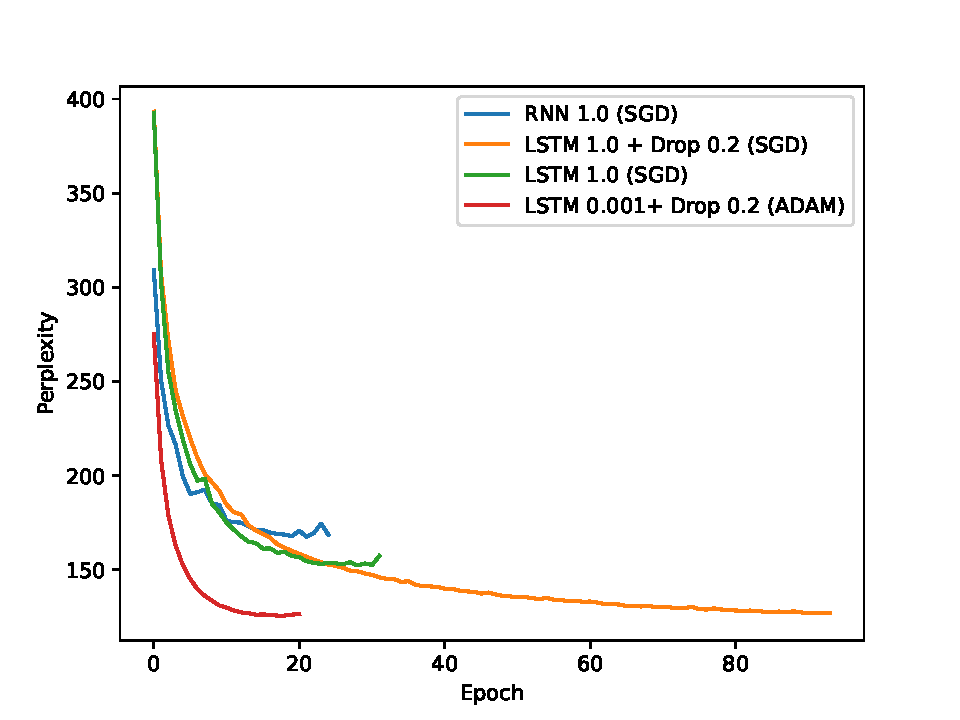
\includegraphics[width=0.5\textwidth]{part1_convergence.pdf}
  \caption{The convergence over the training epochs of selected models in the first part. The labels note the model name with the learning rate, plus if a dropout is applied together the used dropout rate. In parentheses, the optimizer is mentioned. The figure shows that LSTM with dropout and Adam optimizer gives the best results.}
  \label{fig:part_1_convergence}  
\end{figure}

\begin{table}
  \caption{Perplexities in the second part}
  \label{tab:dataPart2}
  \begin{tabular}{l|c c c c c c c}
    \toprule
    \textbf{Model} & \multicolumn{4}{c}{\textbf{Learning rate} } \\
    \midrule
    \textit{SGD optimizer} & \textbf{1.0} & \textbf{2.0} & \textbf{5.0} & \textbf{10.0} & \textbf{20.0} \\
    \midrule
    LSTM      & 106.99  & \underline{104.17}  & 106.22              & 111.32            & 116.35 \\ 
    + WT      & 98.57   & 94.66               & 91.72               & \underline{89.41} & 92.09 \\ 
    + VarDR   & 98.64   & 89.29               & \underline{84.36}   & 84.84             & 95.68 \\ 
    + NT-ASGD & 98.72   & 87.39               & 81.14               & \textbf{79.66}    & 87.62 \\ 
    \bottomrule
  \end{tabular}
  \begin{minipage}{8.5cm}
    \vspace{0.1cm}
    Note: Underlined values show the best perplexity of a model and the bold value shows the best perplexity over all models for a given optimizer. 
  \end{minipage}
\end{table}

\begin{figure}[htbp]
  \centering
  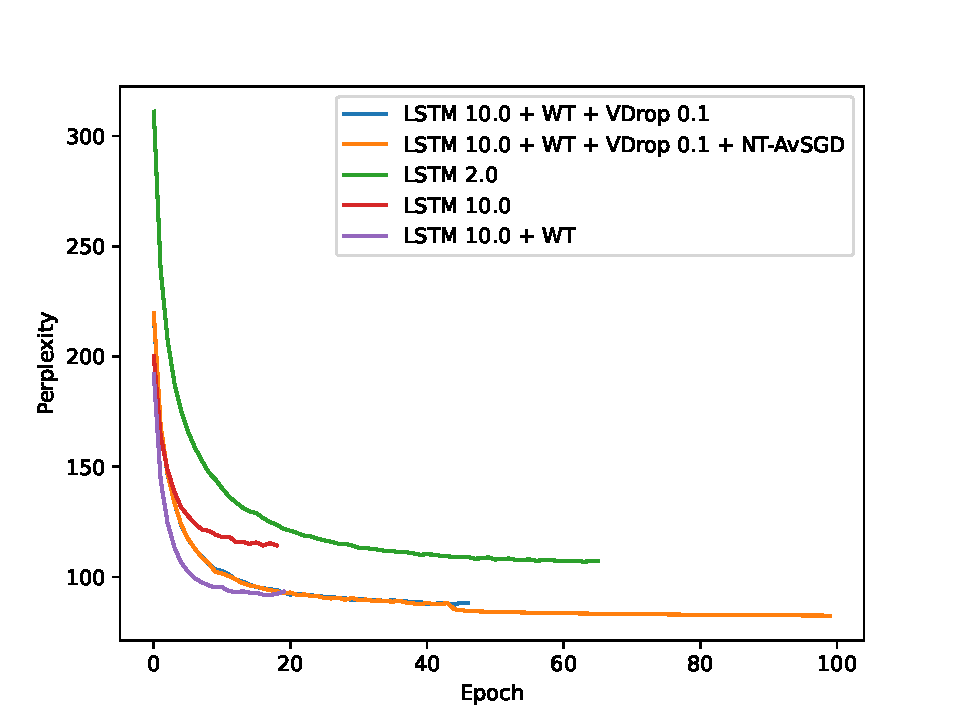
\includegraphics[width=0.5\textwidth]{part2_convergence.pdf}
  \caption{The convergence over the training epochs of selected models in the second part. The labels note the model name with the learning rate, plus which regularization techniques are applied. The figure shows that the LSTM with all regularization techniques gives the best results.}
  \label{fig:part_2_convergence}  
\end{figure}

\bibliographystyle{IEEEtran}

\bibliography{mybib}


\end{document}
